\documentclass{standalone}
\usepackage[utf8]{inputenc}
\usepackage[english]{babel}
\usepackage{tikz}
\usetikzlibrary{positioning}
\begin{document}
  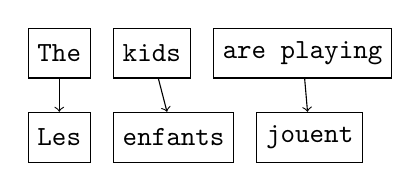
\begin{tikzpicture}[font=\ttfamily] 
    \tikzset{
        block/.style = {rectangle, draw, text centered, minimum height=1.8em, node distance=0.8em},
    }
    \node [block] (a1) {The};
    \node [block,right=of a1] (b1) {kids};
    \node [block,right=of b1] (c1) {are playing};

    \node [block,below=1.2em of a1] (a2) {Les};
    \node [block,right=of a2] (b2) {enfants};
    \node [block,right=of b2] (c2) {jouent};

    \draw[->] (a1) -- (a2);
    \draw[->] (b1) -- (b2);
    \draw[->] (c1) -- (c2);
  \end{tikzpicture}
\end{document}
